\documentclass{../../presentation}

\title{PSE – Vorkurs Tag 3}
\author{Linus, Philipp, Tillmann, Tobias}
\institute{FIUS - Fachgruppe Informatik Universität Stuttgart}
\date{08.09.2025}

\makeatletter
\renewcommand{\lecture@pathprefix}[1]{../../logos/}
\makeatother

\usepackage{todonotes}
\setuptodonotes{inline}
\usepackage{tikz}
\usetikzlibrary{tikzmark}



\begin{document}

\begin{frame}
	\titlepage
\end{frame}

\begin{frame}
	\listoftodos
\end{frame}

\begin{frame}
	\frametitle{Recap Tag 2}
	\todo{am Anfang immer Vortages recap?}
\end{frame}

\begin{frame}[fragile]
	\frametitle{Angenommen \dots}
	\begin{itemize}
		\item\pause Notendurchschnitt von zwei Studis berechnen
		      \begin{minted}{java}
            // Melanie
            double m1 = 1.7, m2 = 2.3, m3 = 1.3;
            double melanieDurchschnitt = (m1 + m2 + m3) / 3;
            System.out.println("Melanies Schnitt: " + melanieDurchschnitt);

            // Paul
            double p1 = 4.0, p2 = 2.3, p3 = 3.3;
            double paulDurchschnitt = (p1 + p2 + p3) / 3;
            System.out.println("Pauls Schnitt: " + paulDurchschnitt);
        \end{minted}
		      \begin{ausgabe}
			      Melanies Schnitt: 1.7666666666666666

			      Pauls Schnitt: 3.1999999999999997
		      \end{ausgabe}
	\end{itemize}
\end{frame}

\begin{frame}[fragile]
	\frametitle{Warum so nicht?!}
	\begin{itemize}
		\item\pause \textbf{Redundanz:} Gleicher Code mehrfach
		\item\pause \textbf{Fehleranfällig:} Zahlendreher möglich
		\item\pause \textbf{Schlecht wartbar:} Änderungen mehrfach nötig
		\item\pause \textbf{Nicht wiederverwendbar:} Nur an dieser Stelle nutzbar
		\item\pause \textbf{Unübersichtlich:} Logik geht unter
	\end{itemize}
	\vspace{2em}
	\begin{minipage}{\textwidth}
		\centering
		\onslide\pause{\Huge $\rightarrow$~}%
		\onslide{\Large Funktionen ermöglichen Wiederverwendung von Code!}
	\end{minipage}
\end{frame}

\begin{frame}[fragile]
	\frametitle{Was sind eigentlich Funktionen?}
	\begin{itemize}
		\item\pause  Möglichket Code auszulagern
		\item\pause Syntax:
		      \begin{minted}{java}   
Rückgabedatentyp Funktionsbezeichner(Datentyp Parametername,...){
        ...
        return Rückgabewert;
 }
        \end{minted}
		\item\pause in unserem Fall:
		      \begin{minted}[fontsize=\footnotesize]{java}
        static void avg(String name, double note1, double note2, double note3) {
            double avg = (note1 + note2 + note3) / 3;
            System.out.println(name + "s Schnitt: " + avg);}
            \end{minted}
	\end{itemize}
	Schlüsselwort \texttt{static} ist hier notwendig wird in PSE genauer erklärt
\end{frame}


\begin{frame}[fragile]
	\frametitle{\texttt{return}}

	\begin{itemize}
		\item\pause Funktionen können Werte zurückgeben
		\item\pause z.B. eine Zahl:
		      \begin{minted}[escapeinside=||]{java}
static |{\tikzmark{rettyp}}|int add(int num1, int num2){
    int sum = num1 + num2;
    return sum;
}
\end{minted}
		\item\pause Datentyp des \texttt{return}-Werts muss im Funktionskopf stehen
		      \begin{tikzpicture}[remember picture, overlay]
			      \draw[->, red, thick]
			      ([yshift=2.5em,xshift=2.5em]pic cs:rettyp)
			      -- ([yshift=1.5ex,xshift=1.0em]pic cs:rettyp)
			      node[anchor=west, yshift=2.0em, xshift=1.0em] {\scriptsize hier \texttt{int} Rückgabetyp};
		      \end{tikzpicture}
		\item\pause Wenn kein Rückgabewert $\rightarrow$ \texttt{void} (wie vorhin)
	\end{itemize}
\end{frame}

\begin{frame}[fragile]
	\frametitle{Verwendung von \texttt{return}}

	\begin{itemize}
		\item\pause Rückgabewert wird zurück an den Aufrufer gegeben
		\item\pause Speicherung in Variable
		      \begin{minted}{java}
int result = add(3, 4);
System.out.println(result); 
		\end{minted}
		      \begin{ausgabe}
			      7
		      \end{ausgabe}
		\item\pause \texttt{return} beendet Funktion sofort
		\item\pause Code nach \texttt{return} wird nicht mehr ausgeführt
	\end{itemize}
\end{frame}


\begin{frame}[plain]
	\centering
	{\Huge\bfseries{Code together}}
	\begin{block}{}
		\[
			\text{Promille} \approx \frac{\text{Alkohol in Gramm}}{\text{Körpergewicht in kg} \times 0{,}65}
		\]
		\[
			\text{Alkohol in Gramm} = \text{Getränkemenge in Liter} \times \text{Vol\%} \times 8
		\]
	\end{block}
\end{frame}

\begin{frame}[fragile]
	\frametitle{Main-Funktion}
	\begin{itemize}
		\item Die \texttt{main}-Funktion ist der Einstiegspunkt für jedes Java-Programm.
		\item Sie wird automatisch aufgerufen, wenn das Programm gestartet wird.
		\item Die \texttt{main}-Funktion muss immer so aussehen:
		      \begin{minted}{java}
public static void main(String[] args) {
    // Hier beginnt das Programm
}
\end{minted}
	\end{itemize}
\end{frame}


\begin{frame}[fragile]{Sichtbarkeit von Variablen (Scopes)}
	\begin{itemize}
		\item\pause Variablen sind sichtbar im aktuellen und in allen tieferen Blöcken
		      \begin{minted}[fontsize=\footnotesize]{java}
public static void main(String[] args) {
int y = 10;

if (y > 5) {
    System.out.println(y); // OK – Zugriff auf äußere Variable
}}
    \end{minted}
		\item\pause In äußeren Blöcken sind sie nicht sichtbar
		      \begin{minted}[fontsize=\footnotesize]{java}
public static void main(String[] args) {
    int x = 5;
}
public static void andereMethode() {
    System.out.println(x); // Fehler! x ist hier nicht sichtbar
}
    \end{minted}

		\item\pause Gilt für alle Blöcke: Funktionen, if, Schleifen, etc.
	\end{itemize}
\end{frame}


\begin{frame}[fragile]
	\frametitle{Basic Scopes}
	\todo{Irgendwas mit dem Meme machen}
	
\includegraphics[width=1\linewidth]{img/scopesmemehoriz.png}
\end{frame}


\begin{frame}[fragile]
	\frametitle{Arrays}
	Mit \textbf{Arrays} kann eine Sammlung von Werten des gleichen Datentyps gespeichert werden.
	\begin{itemize}
		\item Alle Elemente in einem Array müssen den gleichen Datentyp haben (z.\,B.\ \texttt{int}, \texttt{double}, \texttt{String}).
		\item Ein Array hat eine feste Länge, die beim Erstellen festgelegt wird.
		\item Die Elemente im Array sind geordnet und über einen \textbf{Index} erreichbar.
	\end{itemize}
	\begin{minted}{java}
        Datentyp[] Bezeichner = new Datentyp[ArrayLänge];
    \end{minted}
\end{frame}

\begin{frame}[fragile]
	\frametitle{Zugriff auf Elemente eines Arrays}
	\begin{itemize}
		\item Jedes Element hat eine Nummer (index)
		\item Wir können über den Index auf die Elemente zugreifen
	\end{itemize}
	\begin{columns}
		\column{0.5\linewidth}
		\begin{minted}{java}
            int[] array = new int[5];
            array[0] = 6;
            array[2] = 9;
        \end{minted}

		\column{0.5\linewidth}
		\begin{center}
			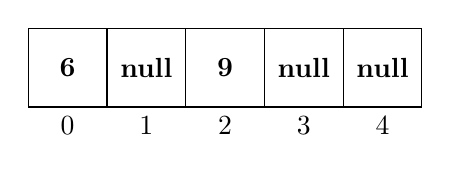
\begin{tikzpicture}
				\foreach \x in {0,1,...,4} {
						\draw (\x,0) rectangle coordinate(c\x) (\x+1, 1);
						\node[below] at (\x+0.5, 0) {\x};
					}
				\node at (c0) {\bf 6};
				\node at (c1) {\bf null};
				\node at (c2) {\bf 9};
				\node at (c3) {\bf null};
				\node at (c4) {\bf null};
			\end{tikzpicture}
		\end{center}
	\end{columns}

	\vspace{0.5cm}

	\begin{itemize}
		\item Die Array-Variable speichert die Länge das arrays: \mintinline{java}{array.length}
		\item Der höchste Index ist immer \mintinline{java}{array.length - 1}
	\end{itemize}
\end{frame}

\begin{frame}[fragile]
	\frametitle{Arrays}
	Wir können Arrays auch direkt mit Werten initialisieren
	\begin{minted}{java}
    String[] grillSachen = {"würstchen", "steak", 
                            "grillkäse", "maiskolben"};
    \end{minted}
	Und wir können sie auch mit einer Schleife durchlaufen:
	\begin{minted}{java}
    System.out.println(grillSachen[1]);
    for (int i = 0; i < grillSachen.length; i++) {
        System.out.println(grillSachen[i]);
    }
    \end{minted}
\end{frame}

\end{document}
